\documentclass{article}
\usepackage[utf8]{inputenc}
\usepackage{hyperref}
\usepackage{amsmath}
\usepackage{graphicx}


\graphicspath{ {./images/} }
\setlength\parindent{0pt}

\title{Reinforcement Learning}
\author{Bart Lammers}
\date{May 2022}

\begin{document}

\maketitle

\tableofcontents
\clearpage

\section{Markov Decision Process}

\begin{itemize}
    \item $S$: state space $s_0, s_1, s_2$
    \item $P_0$: starting state distribution
    \item $A$: Action space $a_0, a_1, a_2$
    \item $P$: transition function $P(s_{t+1}|a_t, s_t)$
    \item $R$: reward function $R(s_t, a_t, s_{t+1})=r_t$
\end{itemize}

\section{RL concepts}

\textbf{Policy}

\begin{itemize}
    \item Sample the action to take from the policy function given the state
    \item $\mu(s_t) \rightarrow a_t$: deterministic
    \item $a_t \sim \pi(s_t)$: stochastic
\end{itemize}

\textbf{Episode} / roll-out / trajectory

\begin{itemize}
    \item The history (states and actions) of a single run
    \item $\tau = [s_0, a_0, s_1, a_1, s_2, a_0, ...]$
\end{itemize}

\textbf{Return}

\begin{itemize}
    \item Cumulative reward in a trajectory
\end{itemize}

\section{RL course David Silver}

\href{https://www.davidsilver.uk/teaching/}{Link to teaching material}

\section{Lecture 1 - introduction}

\subsection{RL problem}

\textbf{Agent and environment}

At each step $t$ the agent:
\begin{itemize}
    \item Executes action $A_t$
    \item Receives observation $O_t$
    \item Receives scalar reward $R_t$
\end{itemize}

At each step $t$ the environment:
\begin{itemize}
    \item Receives action $A_t$
    \item Emits observation $O_t$
    \item Emits scalar reward $R_t$
\end{itemize}

This interaction between agent and environment yields a stream of data which is the experience of the agent and the data that the reinforcement learning problem is concerned with.\\

\textbf{History} - $H_t = A_1, O_1, R_1, ..., A_t, O_t, R_t$

\begin{itemize}
    \item $A$: action
    \item $O$: observation
    \item $R$: reward
\end{itemize}

History determines what happens next but isn't very useful. More useful is \textbf{state}: a summary of the history that contains the information that determines what happens next. The state is a function of the history $S_t = f(H_t)$ \\

Three different versions of state:
\begin{itemize}
    \item Environment state $S_t^e$: information private to the environment that captures it's state, whatever it uses to pick the next observation / reward
    \item Agent state $S_t^a$: agents internal representation used to pick the next action. Can be any function of the history - we can constrcut this state based on what we need!
    \item Information state / Markov state / sufficient statistic: contains all useful information from the history. A state is Markov if and only if: $P[S_{t+1}|S_t] = P[S_{t+1}| S_1, ..., S_t]$ (future is independent of the past given the present)
\end{itemize}

\textbf{Observability}
\begin{itemize}
    \item Full observability: $O_t=S_t^a=S_t^e$ - this is a Markov Decision Process (MDP)
    \item Partial observability $S_t^a \neq S_t^e$ - this is a partially observable MDP - agent must construct it's own state. Examples:
    \begin{itemize}
        \item Complete history (naive)
        \item Beliefs on environment state (Bayesian approach) - probability distribution over the states
        \item Recurrent neural network: linear combination of new observation $O_t$ and the previous state $S_{t_1}^a$ followed by a non-linearity
    \end{itemize}
\end{itemize}

\subsection{RL agent components}

An agent may contain the following components:
\begin{itemize}
    \item Policy: agent behavior - mapping from state to action 
    \begin{itemize}
        \item Deterministic: $a=\pi(s)$
        \item Stochastic: $\pi(a|s)=P[A=a|S=s]$
    \end{itemize}
    \item Value function: prediction of expected future reward - mapping from state and action to reward
    \begin{itemize}
        \item Depends on your policy. Value function is always FOR a policy
        \item $v_\pi(s)=E_\pi[R_t+\gamma R_{t+1} + \gamma^2R_{t+2} + ... | S_t=s]$
        \item Basis for good decisions because it allows to compare different possible actions based on the expected future rewards that they are going to yield
    \end{itemize}
    \item Model: predicts what the environment will do next
    \begin{itemize}
        \item This is optional, there are a lot of "model-free" models
        \item We break this up into Transitions and Rewards (immediate rewards)
        \item Transitions: $\mathcal{P}^a_{ss'}=P[S'=s'|S=s, A=a]$
        \item Rewards: $\mathcal{R}^a_{s}=P[R|S=s, A=a]$
    \end{itemize}
\end{itemize}

\textbf{Categorizing RL agents}\\

Based on policy / value function
\begin{itemize}
    \item Value based
    \begin{itemize}
        \item No policy - policy is implicit, it just reads out the value function and picks the action that yields the highest value
        \item Has a value function
    \end{itemize}
    \item Policy based
    \begin{itemize}
        \item Has a policy - directly determines actions based on state, not through expected values 
        \item No value function
    \end{itemize}
    \item Actor critic
    \begin{itemize}
        \item Combines both together
        \item Has a policy and a value function
    \end{itemize}
\end{itemize}

Based on model / model-free

\subsection{Key problems within RL}

\textbf{Sequential decision making} - two fundamental problems
\begin{itemize}
    \item Reinforcement learning - environment is unknown initially and the agent learns about it by interacting - trial and error
    \item Planning - we know the environment upfront
    \item These problems are intimately linked. It is not uncommon to first do reinforcement learning and then, once the environment is known, do planning
\end{itemize}

\textbf{Exploration vs exploitation}
\begin{itemize}
    \item Exploration learns more about the environment
    \item Maximize rewards using the information you have already collected
\end{itemize}

\textbf{Prediction and control}
\begin{itemize}
    \item Prediction: evaluate the future (given a policy, how well will I do)
    \item Control: optimize the future (find the best policy)
    \item Typically we need to solve the prediction problem to then solve the control problem
\end{itemize}

\section{Lecture 2 - Markov Decision Processes}

\textbf{Lecture outline}
\begin{itemize}
    \item Markov processes / Markov chains: vanilla
    \item Markov reward processes: adding reward in
    \item Markov decision processes: adding actions in
\end{itemize}

\subsection{Markov processes}
\begin{itemize}
    \item Markov property: current state captures all required information, rest of history can be thrown away
    \item State transition matrix $\mathcal{P}_{ss'}=P[S_{t+1}=s'|S_t=s]$
    \item Markov process $(\mathcal{S}, \mathcal{P})$: memoryless random process, ie. a sequence of random states. It is defined by:
    \begin{itemize}
        \item $\mathcal{S}$ - a finite set of states
        \item $\mathcal{P}$ - a transition probability matrix
    \end{itemize}
\end{itemize}
    
\subsection{Markov Reward Processes}

\begin{itemize}
    \item Markov reward process $(\mathcal{S}, \mathcal{P}, \mathcal{R}, \gamma)$: Markov chain with value judgements (how much reward have I accumulated across this path). In RL we care about maximising the cumulative rewards over time!
    \begin{itemize}
        \item $\mathcal{R}$ - reward function $\mathcal{R}_s=E[R_{t+1}|S_t=s]$, $R_t$ is the immediate reward at single moment. This function tells us, given that we are in state $s$, how much reward will we receive in the next timestamp
        \item $\gamma$ - discount factor
    \end{itemize}
    \item Example of the student Markov chain (three classes, can get distracted by Facebook or the pub), with the Markov reward process we now add values to each state, which are assigned when you enter the state (pass course: +10, take class: -2, go to pub: +3)
    \item \textbf{Return} $G_t=R_{t+1}+\gamma R_{t+2}+...=\sum^\infty_{k=0}\gamma^k R_{t+k+1}$ is the total discounted reward from time step $t$ onwards - can be thought of as the goal, it's what we try to optimize. Using the discount factor $\gamma$ we make it finite
    \item Why discount?
    \begin{itemize}
        \item Because there is more uncertainty into the future, make the model focus on things in its span of control
        \item Because it is mathematically convenient to have a finite metric
    \end{itemize}
    \item \textbf{Value function} $v(s)=E[G_t|S_t=s]$ - gives the long-term value of state $s$
    \begin{itemize}
        \item In other words: expected return starting from state $s$
        \item Central quantity we are interested in within RL
        \item Can estimate by sampling episodes from a MDP. Then for a certain state $s$ calculating the return of each episode. The estimate for the value function is the average of the returns
    \end{itemize}
    \item Bellman equation - the value function $v(S_t)$ can be decomposed into two parts:
    \begin{itemize}
         \item Immediate reward $R_{t+1}$
         \item Discounted value of next state $\gamma v(S_{t+1})$
         \item Matrix notation: $v=\mathcal{R} + \gamma \mathcal{P}v$, where $v$ is a column vector with each element corresponding to a state, $\mathcal{R}$ is a column vector of immediate rewards and $\mathcal{P}$ is the transition probability matrix
         \item $v(s)=\mathcal{R}_s+\gamma \sum_{s'\in \mathcal{S}}\mathcal{P}_{ss'}v(s')$ - can be seen as a "one step look ahead" / one step tree. This is a convenient thing to memorize as we'll also use it during computation: we sum the immediate reward and the weighted average (weights are the probabilities) of the value function outputs in the next states
         \item Evaluating the rewards can be solved directly for small MDPs since it's a linear equation: $v=(I - \gamma \mathcal{P})^{-1} \mathcal{R}$ with computational complexity $O(n^3)$ due to inverting a matrix with dimensions equal to the transition probability matrix. If we want to maximize rewards (Markov Decision Processes) we cannot solve it anymore analytically
    \end{itemize}
\end{itemize}

\subsection{Markov Decision Processes}

\begin{itemize}
    \item Markov Decision Processes $(\mathcal{S}, \mathcal{A}, \mathcal{P}, \mathcal{R}, \gamma)$ is a Markov reward process with decisions (so adding one more level of complexity: actions $\mathcal{A}$)
    \begin{itemize}
        \item $\mathcal{A}$ is a finite set of actions
        \item The state transition matrix now depends on which action we take: $\mathcal{P}_{ss'}^a=P[S_{t+1}=s'|S_t=s, A_t=a]$
        \item The reward function may now depends on the action we take: $\mathcal{R}_s^a=E[R_{t+1}|S_t=s, A_t=a]$
        \item Now, in the student MDP example, rather than having all random transitions (according to the probabilities), the agent has some control. It can choose actions in certain states (eg. "study", "Facebook"), but some states still have only random transitions ("if you go to the pub, anything might happen")
    \end{itemize}
    \item \textbf{Policy} $\pi(a|s)=P[A_t=a|S_t=s]$ is a distribution over actions given state. It is a mapping of state to action. It fully defines the behavior of the agent. Due to the Markov property, policies are stationary (time-independent)
    \item Side note: for any Markov Decision Process, if we fix the policy, we can always "flatten" it into a Markov Process or a Markov Reward Process
    \item \textbf{Value function} - now we have two value functions:
    \begin{itemize}
        \item The \textit{state-value function}
        \begin{equation}
            v_\pi(s)=E_\pi[G_t|S_t=s]
        \end{equation} 
        now depends on the policy $\pi$ - it's the expected return, starting from state $s$, and then following the policy
        \item The \textit{action-value function}
        \begin{equation}
            q_\pi(s, a)=E_\pi[G_t|S_t=s, A_t=a]
        \end{equation}
        is the key quantity we are going to use to determine the best actions! It's the expected return, starting from state $s$, taking action $a$, and then following the policy
    \end{itemize}
    \item Bellman equations for these value functions, again the same decomposition using recursion:
    \begin{itemize}
        \item State-value function: 
        \begin{equation}
            v_\pi(s)=E_\pi[R_{t+1}+\gamma v_\pi(S_{t+1})|S_t=s]
        \end{equation}
        \item Action-value function: 
        \begin{equation}
            q_\pi(s, a)=E_\pi[R_{t+1}+\gamma q_\pi(S_{t+1}, A_{t+1})|S_t=s, A_t=a]
        \end{equation}
    \end{itemize}
    \item Averaging over states and actions allows us to estimate these quantities (\textbf{lecture minute 50}: useful intuitive explanation on these decompositions using look-ahead trees):
    \begin{itemize}
        \item State-value function:
        \begin{equation}
            v_\pi(s)=\sum_{a\in \mathcal{A}}\pi(a|s)q_\pi(s, a)
        \end{equation}
        in words: "average over the actions that we might take" - if we are in state $s$ now, then we take the weighted average of the expected return over all the actions (given by the action-value function $q_\pi(s,a)$), where the weights are the probabilities of taking each action (given by the policy $\pi(a|s)$)
        \item Action-value function:
        \begin{equation}
            q_\pi(s, a)=\mathcal{R}^a_s+\gamma \sum_{s'\in \mathcal{S}}\mathcal{P}^a_{ss'}v_\pi(s')
        \end{equation}
        in words: "average over the states we might end up in" - if we are in state $s$ now and take action $a$, then sum the immediate reward for taking the action ($\mathcal{R}^a_s$), to the weighted average (weights given by the transition matrix $\mathcal{P}^a_{ss'}$) of values of the states (given by $v_\pi(s')$) we might end up in after taking action $a$
        \item State-value function - stitching together (recursive relation that allows us to understand $v$ in terms of itself, "this is how we end up solving MDPs"): 
        \begin{equation}
            v_\pi(s)=\sum_{a\in \mathcal{A}}\pi(a|s) \left( \mathcal{R}^a_s+\gamma \sum_{s'\in \mathcal{S}}\mathcal{P}^a_{ss'}v_\pi(s') \right)
        \end{equation} 
        in words: averaging over both all the actions we might take (the policy gives us the probabilities of the actions) and what the environment might do to us (transition probability matrix gives us the probabilities for each next state given the action)
        \item Action-value function - stitching together (recursive relation that allows us to understand $q$ in terms of itself, "this is how we end up solving MDPs"):
        \begin{equation}
            q_\pi(s, a)=\mathcal{R}^a_s+\gamma \sum_{s'\in \mathcal{S}}\mathcal{P}^a_{ss'}\sum_{a'\in \mathcal{A}}\pi(a'|s')q_\pi(s', a')
        \end{equation}
    \end{itemize}
    \item Solving an MDP: what is the optimal path (evolution) that will lead to the maximal reward in expectation?
    \begin{itemize}
        \item Optimal state-value function: $v_*(s)=\underset{\pi}{\text{max }}  v_\pi(s)$ --- does not yet tell you how to behave --- in the example student-MDP, this function tells you what value each of the states (nodes) have
        \item Optimal action-value function: $q_*(s, a)=\underset{\pi}{\text{max }} q_\pi(s, a)$ --- this one tells you, if I am in state $s$ and I take next action $a$, what is the expected maximum reward I can get from then on wards. If you have this one you can iterator over the actions and pick the one with the highest maximum expected reward --- in the example student-MDP, this function tells you the value of each action (edges) 
    \end{itemize}
    \item \textbf{Optimal policy theorem} - ``sanity check'', what you hoped was true is true - $\pi \geq \pi'$ if $v_\pi(s) \geq v_{\pi'}(s), \forall s$ - for any MDP:
    \begin{itemize}
        \item There exists an optimal policy, that is better than or equal to all other policies, $\pi_* \geq \pi, \forall \pi$
        \item All optimal policies achieve the optimal value function, $v_{\pi_*}(s)=v_*(s)$
        \item All optimal policies achieve the optimal action-value function, \\$q_{\pi_*}(s, a)=q_*(s, a)$
    \end{itemize}
    \item Finding an optimal policy: at each step pick the action that maximizes $q_*(s, a)$ --- there is always a deterministic optimal policy for any MDP
    \begin{equation}
        \pi_*(a|s)=
        \begin{cases}
            1 &\text{if } a=\underset{a \in \mathcal{A}}{\text{argmax }} q_*(s, a) \\
            0 &\text{otherwise}
        \end{cases}
    \end{equation}
    \item \textbf{Bellman Optimality Equation} - this is the equation generally know as the Bellman equation - ``this one tells you how to really solve your MDP'' - shows how to relate the optimal value functions to itself by recursion - again intution is the one-step look-ahead charts
    \begin{itemize}
        \item For the state-value function - instead of before taking the average, we now take the action that maximizes the $q$ value:
        \begin{equation}
            v_*(s)=\underset{a}{\text{max }}q_*(s, a)
        \end{equation}
        \item For the action-value function - incorporates chance, ``where the wind may take us'', where will the environment take us next - so here we're averaging over transition probabilities again:
        \begin{equation}
            q_*(s, a)=\mathcal{R}^a_s+\gamma \sum_{s'\in \mathcal{S}}\mathcal{P}^a_{ss'}v_*(s')
        \end{equation}
        \item Putting those together to get to recursive equation for $v_*$ -- two step look-ahead, first over actions (taking the max) then over states we might end up in (averaging over transition probabilities)
        \begin{equation}
            v_*(s)=\underset{a}{\text{max }} \left( \mathcal{R}^a_s+\gamma \sum_{s'\in \mathcal{S}}\mathcal{P}^a_{ss'}v_*(s') \right)
        \end{equation}
        \item Similarly to get to a recursive equation for $q_*$ -- two step look-ahead, first over transition probabilities in the environment, then over the best actions ($\underset{a'}{\text{max }}q_*(s', a')$) we might take from there
        \begin{equation}
            q_*(s, a)=\mathcal{R}^a_s+\gamma \sum_{s'\in \mathcal{S}}\mathcal{P}^a_{ss'}\underset{a'}{\text{max }}q_*(s', a')
        \end{equation}
        \item How do we solve these Bellman equations now? These functions are now non-linear due to taking the max, so there is no close-form solution. Now we need to resolve to dynamic programming solution that solve it iteratively:
        \begin{itemize}
            \item Value iteration
            \item Policy iteration
            \item Q-learning
            \item Sarsa
        \end{itemize}
        \item Extensions to MDPs not discussed in this class:
        \begin{itemize}
            \item Infinite and continuous MDPs (eg. continuous actions, continuous timestamps)
            \item Partially observable MDPs
            \item Undiscounted, average reward MDPs
        \end{itemize}
    \end{itemize}
\end{itemize}

\section{Lecture 3 - Dynamic Programming}

\textbf{Lecture outline}
\begin{itemize}
    \item Introduction
    \item Policy evaluation
    \item Policy iteration
    \item Value iteration
    \item Extensions to dynamic programming
    \item Contraction mapping
\end{itemize}

\subsection{Introduction}

\begin{itemize}
    \item Policy evaluation, policy iteration and value iteration are three major paradigms. In the next lectures we will ``pull'' ideas from these areas and develop them into functional tools we can use in RL
    \item \textbf{Dynamic programming}
        \begin{itemize}
            \item \textbf{Dynamic}: sequential / temporal / step-by-step component to the problem
            \item \textbf{Programming}: from the ``optimizing a program'' perspective (like linear programming)
            \item It's a method of solving complex problems by breaking them into sub-programs and solving those, then putting them back together
        \item Dynamic programming can apply to problems with two properties:
        \begin{itemize}
            \item Optimal substructure: optimal solution can be decomposed into sub-problems
            \item Overlapping sub-problems: sub-problems recur many times (\textbf{so that we can cache and re-use solutions})
        \end{itemize}
        \item MDPs satisfy both through the Bellman equations. The recursive nature of the value function enables storing and re-using solutions
    \end{itemize}
    \item Today we are going to use dynamic programming to solve the MDP, and assume full knowledge of the MDP (``someone tells us the transition and reward structure''). This makes it a \textbf{planning} problem --- this is not yet ``full reinforcement learning''
    \item Can be used for:
    \begin{itemize}
        \item Prediction / policy evaluation: input MDP $\langle\mathcal{S}, \mathcal{A}, \mathcal{P}, \mathcal{R}, \gamma \rangle$ and policy $\pi$ - output: value function $v_\pi$
        \item Control / optimization: input MDP $\langle\mathcal{S}, \mathcal{A}, \mathcal{P}, \mathcal{R}, \gamma \rangle$ - output: optimal value function $v_*$ and optimal policy $\pi_*$
    \end{itemize}
\end{itemize}

\subsection{Policy evaluation}

\begin{itemize}
    \item Problem: ``prediction'' - evaluate a given policy $\pi$ (in other words: what is the value function $v_\pi$?)
    \item Solution: iterative application of \textbf{Bellman expectation equation} in a backup computation
    \item Synchronous back-up: at each iteration update all states using Bellman equation (for each state doing a one-step look ahead), and then continue with next iteration. Is proven to converge to $v_\pi$. Update: $\mathbf{v}^{k+1}=\mathbf{\mathcal{R}^\pi} + \gamma\mathbf{\mathcal{P}^\pi}\mathbf{v}^k$ (matrix notation)
    \item Example with small Small Gridworld, finding out the number of steps to a terminal state by setting the reward from each state to the next to -1, \textbf{given} a policy of taking a step up, down, left or right all with 0.25 probability:
    \begin{itemize}
        \item Starting point for the iterative process is to set a naive value (in this case zero) as the value for each state - it does not matter where you start
        \item By iteratively computing the next values for states from the previous value and the values from the bordering states (doing one-step look-aheads) the values converge to the true value function given the policy $\pi$
        \item Moving towards policy iteration: if we now instead set a greedy policy on these estimate of the value function (always go to the state with the highest value), we see that we quickly arrive at the optimal policy (easy to see from the example), even though we have approximated the value function for a different policy (the random one), and we have only taken three iteration steps. Intuition is that we can use the value function which has been approximated for a different policy to build a new policy that is better than the previous one, by acting greedily
    \end{itemize}
\end{itemize}

\subsection{Policy iteration}

\begin{itemize}
    \item Problem: ``control'' - determine the optimal policy given the rewards and the system dynamics (transition probabilities)
    \item Solution: iterative application of \textbf{Bellman expectation equation} followed by a \textbf{greedy policy improvement}
    \item Given a policy $\pi$, iteratively:
    \begin{enumerate}
        \item \textbf{Evaluate} the policy $v_\pi(s)=E[R_{t+1} + \gamma R_{t+2} + ... | S_t=s]$
        \item \textbf{Improve} the policy by acting greedily wrt. $v_\pi$ (in each state taking the action that maximizes the value function)
    \end{enumerate}
    \item This process always iterates to the optimal policy $\pi_*$. 
    \item This concept of repeated (1) evaluation of the value function given a policy and then (2) improvement to by acting greedily on the new estimated value function is used again and again in RL. Guaranteed to converge to the optimal value function $v_*$ and the optimal policy $\pi_*$
    \item You can do multiple iterations of step 1 and then a single step 2 in each iteration. If you do a single step 1 (evaluate) followed by a single step 2 (improve), it relates closely to value iteration.
\end{itemize}

\subsection{Value iteration}

\begin{itemize}
    \item Problem: ``control'' - determine the optimal policy given the rewards and the system dynamics (transition probabilities)
    \item Solution: iterative application of the \textbf{Bellman optimality equation}
    \item Note: still, we are doing ``planning'' and not solving the full RL problem since we see the rewards and transition probabilities as given
    \item Value iteration works ``directly in value space'' by iteratively applying the Bellman optimality equation
    \begin{itemize}
        \item It converges to the value function for the \textbf{optimal policy}
        \item It does not build the policy as an intermediate step. In value iteration you do a single evaluate step, followed by a single greedy improve step over the new value function (argmax in policy iteration gives you the policy, which step to take), but it does so in a single step (by taking a max, giving the next optimal value)
        \item There is no explicit policy, and in intermediate steps it may not correspond to any policy, they are just intermediate constructs
    \end{itemize}
\end{itemize}

\subsection{Extensions to dynamic programming}

\begin{itemize}
    \item Asynchronous dynamic programming allows to decrease computation cost by selecting which states to update in some way. This still converges to the correct solution as long as all states are still being selected
    \item Some flavours:
    \begin{itemize}
        \item In-place value iteration: don't wait until you have updated the value function for all states, instead just always use the latest values from bordering states, also if they have been updated just before in the current evolution. With some ordering tricks this can be much more efficient
        \item Prioritised sweeping: come up with a ``priority'' metrics that says how important it is to update a state in the MDP? The magnitude of the change in the Bellman equation in the last state updates.
        \item Real-time dynamic programming: select the states that the agent actually visits when you apply the agent in the environment (``real world'')
    \end{itemize}
    \item Dynamic programming, due to it's ``full width back-ups'' suffers from Bellman's curse of dimensionality: the number of states grows exponentially with the number of states. To make this more efficient we can instead sample the back-ups from the dynamics from the environment. This also opens the door for model-free RL because instead of knowing the dynamics, we just sample from them
\end{itemize}

\section{Lecture 4 - Model-Free Prediction}

\textbf{Lecture outline}

\begin{itemize}
    \item Introduction
    \item Monte-carlo learning
    \item Temporal-difference learning
    \item TD($\lambda$)
\end{itemize}

Very useful slides - not everything is captured in this summary

\subsection{Introduction}

\begin{itemize}
    \item Explanation \textbf{model free}: so far, we looked at MDPs for which we knew the rewards and dynamics (transition probabilities) given. Now we consider the case where we don't exactly know how the system works ``no one tells us about the environment and the agent still needs to learn how to behave optimally''.
    \item Monte-carlo methods: complete a full trajectory and estimate the reward of the trajectory summing the sample returns in the steps
    \item Temporal-difference methods: look one step ahead and then estimate the total reward of the trajectory, can be much more efficient
    \item TD($\lambda$) - unification of the above two methods where we can take any number of steps and then estimate
    \item Overview of last / this / next lecture:
    \begin{itemize}
        \item Last lecture: planning by dynamic programming - solving \textbf{known} MDPs (known reward function and known dynamics)
        \item This lecture: model-free prediction - estimating the value function for \textbf{unknown} MDPs, given a policy
        \item Next lecture: model-free control - optimise the value function for \textbf{unknown} MDPs, and therefore find the optimal policy
    \end{itemize}
\end{itemize}

\subsection{Monte-Carlo reinforcement learning}

\begin{itemize}
    \item Goal: learn $v_\pi$ (expected future return from every state under policy $\pi$) from episodes of experience under policy $\pi$ 
    \item MC is efficient and widely used in practice and is a simple idea that allows for full RL
    \item Looks at complete episodes, episode must always terminate (``only works for episodic MDPs''). Looks at sample returns to estimate the value function (empirical mean return from each state onwards is the estimate for the value function)
    \item In these model-free methods, we depend on sampling rather than full sweeps over all states (like in dynamic programming). This is nice because it means that the computation does not depend on the size of the state space any more
    \item In this lecture we are evaluating a policy, which means we only care about the states that are visited by the policy. In the next lecture, we will discuss optimization. Which means we consider if the policy needs to visit new states and check if it increases our value function. This is the problem of exploration which is a central problem in RL and will be a topic when we discuss optimization only
    \item Only issue is how do we estimate $v$ for all states if we only have trajectories and can't pick which states we'll visit? Two different solutions:
    \begin{itemize}
        \item First-visit MC policy evaluation: per state, keep track of 1) the number of visits to that state, and 2) the total return collected across episodes in that state. Then value is estimated by the mean return (sum of returns divided by the number of visits). Note: the counter and total value are only incremented the \textbf{first time} the state is visited per episode
        \item Every-visit MC policy evaluation: similar to first-visit, but now we increment the total return accumulated in the state and the counter in every state visit in the episode (not just in the first visit). Otherwise identical to first-visit. Both are valid estimators
    \end{itemize}
    \item These methods can also be used online by computing the mean incrementally after each episode (when we have the return of the episode)
    \begin{equation}
        \mu_k = \mu_{k-1}+\frac{1}{k}(x_k-\mu_{k-1})
    \end{equation}
    we'll see many algorithms that use an update statement similar to this
    \item For Monte-Carlo methods we can use the following incremental updates (after each episode, when we have the return $G_t$, this way we don't need to maintain old returns and just update the statistics)
    \begin{equation*}
        N(S_t) \leftarrow N(S_t) + 1 
    \end{equation*}
    \begin{equation*}
        V(S_t) \leftarrow V(S_t) + \frac{1}{N(S_t)}(G_t-V(S_t)) 
    \end{equation*}
    \item \textbf{In the real world}, things can drift around (it's a non-stationary problem), there you always need to forget old episodes by tracking a running mean. You do this by having a constant step size $\alpha$ (this is an exponential moving average):
    \begin{equation}
        V(S_t) \leftarrow V(S_t) + \alpha(G_t-V(S_t)) 
    \end{equation}
\end{itemize}

\subsection{Temporal-Difference learning}

\begin{itemize}
    \item Goal: still policy evaluation (learn $v_\pi$ online from experience), next class we'll see how we can use TD for control
    \item Simplest temporal-difference learning algorithm: TD(0)
    \begin{itemize}
        \item Update $V(S_t)$ towards the estimated return $R_{t+1}+\gamma V(S_{t+1})$:
        \begin{equation}
            V(S_t) \leftarrow V(S_t) + \alpha(R_{t+1}+\gamma V(S_{t+1})-V(S_t)) 
        \end{equation}
        \item Difference with every-visit MC is that we substitute the empirical sampled reward $G_t$ with the \textit{TD target} $R_{t+1}+\gamma V(S_{t+1})$
        \item The estimated return / TD target again consists of two parts (like in the Bellman equations):
        \begin{itemize}
            \item $R_{t+1}$ - immediate reward
            \item $\gamma V(S_{t+1})$ - discounted value of the next step
        \end{itemize}
    \end{itemize}
    \item Intuition into why TD works, where does it get it's real-world signal from? Every step you get real rewards from the environment, and the dynamics of the environment affect the state you and up in after you take a certain action. These rewards and dynamics are sampled from the environment and therefore ``ground'' you in the real-world, and every update step makes the estimated value function approximate the true value function closer and closer
    \item \textbf{Bootstrapping}:
    \begin{itemize}
        \item Allows learning from incomplete episodes - you update a value function for a state only based on the output of the value function for the surrounding states
        \item TD ``updates a guess towards a guess'' - intuition: start of by guessing the full reward at the begin of the episode (evaluate value function), take a couple of steps, then guess again (evaluate value function), then update the original guess towards you substitute guess
        \item MC does not bootstrap (instead it completed the full episode and uses the sampled return to update the value function for the current state)
        \item Dynamic programming bootstraps (using the updates defined by the Bellman equations)
        \item TD bootstraps
    \end{itemize}
    \item \textbf{Sampling}
    \begin{itemize}
        \item MC samples
        \item Dynamic programming does not sample (calculates the expected values given the rewards and transition probabilities)
        \item TD samples
    \end{itemize}
    \item TD method, compared to Monte Carlo:
    \begin{itemize}
        \item Also learns directly from episodes of experiences
        \item Also is model-free (MDP transitions and rewards unknown)
        \item Contrary to Monte Carlo, it learns from \textit{incomplete} episodes, by bootstrapping (guessing the remaining reward instead of fully completing the episode) therefore it can also learn without the final outcome (incomplete sequence) whereas MC can't
        \item TD works in continuing (non-terminating) environments whereas MC only works for episodic (terminating) environments
        \item TD learns online after every step, MC must wait until the end of the episode when the return is known
        \item Intuitive example: let's say you are in a car and almost crash into an other car but in the last second the crash is averted. In MC, you would still arrive at your target and get a positive reward, and you would not be able to learn from this near-death experience. In TD, your estimate of the total reward you were going to get would reflect the near-crash situation, since it would be very negative just before the crash. This would allow you to learn (maybe I should have slowed down a bit earlier) without actually crashing the car
        \item Good example of difference in the updates in the ``driving home example'' (minute 41):
        \begin{figure}[h]
            \centering
            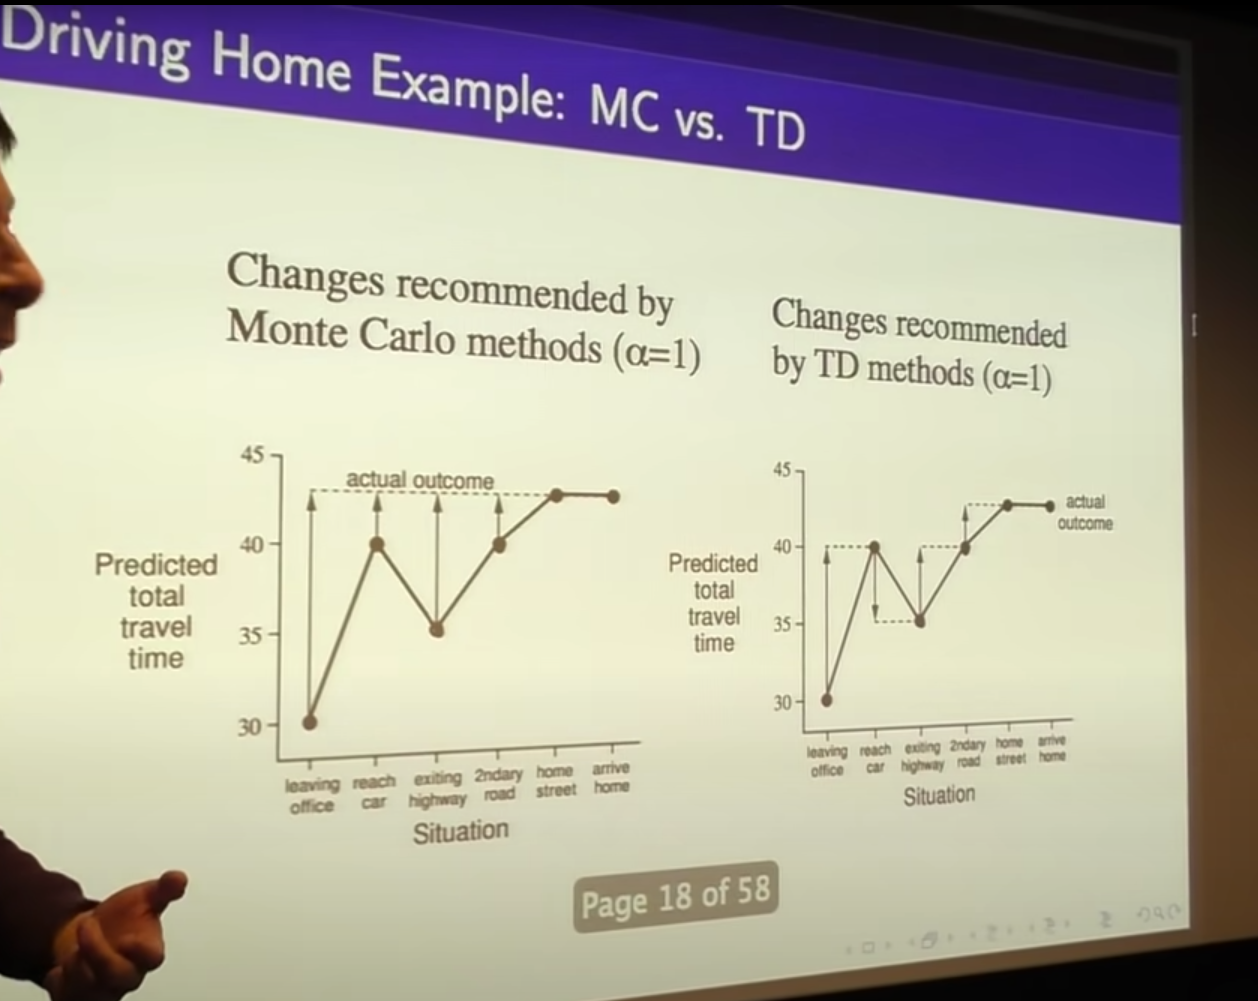
\includegraphics[scale=.2]{td_mc_driving_home}
        \end{figure}
        \item Bias / variance trade-off:
        \begin{itemize}
            \item Return used in MC is $G_t=R_{t+1}+\gamma R_{t+2} + ... + \gamma^{T-1}R_T$ (sample of the actual returns) which is an unbiased estimator of $v_\pi(S_t)$
            \item For TD:
            \begin{itemize}
                \item If we would use the true TD target $R_{t+1}+\gamma v_\pi(S_{t+1})$ it would be an unbiased estimator of $v_\pi(S_t)$ - but we don't have the true value function $v_\pi(S_{t+1})$
                \item Instead we use $R_{t+1}+\gamma V(S_{t+1})$ which is a biased estimator of $v_\pi(S_t)$ but with much lower variance - the variance is lower because $V(S_{t+1})$ is just a fixed function, which you evaluate and returns a single number, whereas the sampled returns contain a lot of variation because there are a lot of steps where the environment can have a lot of random influence (due to actions, transitions, rewards) - ``we're only looking at the variance included in the first step (due to the single $R_{t+1}$ term) and not over the whole trajectory''
            \end{itemize}
        \end{itemize}
        \item MC has high variance, zero bias - directly copied from slide:
        \begin{itemize}
            \item Good convergence properties
            \item (even with function approximation) (Note: in later lectures we'll see that determining the value function is impractical because there are so many states, so instead we'll use function approximator for it)
            \item Not very sensitive to initial value
            \item Very simple to understand and use
        \end{itemize}
        \item TD has low variance, some bias - directly copied from slide:
        \begin{itemize}
            \item Usually more efficient than MC
            \item TD(0) converges to $v_\pi(s)$
            \item (but not always with function approximation)
            \item More sensitive to initial value
        \end{itemize}
        \item TD exploits Markov property (the current state is all you need) by implicitly building the Markov property, which makes it more efficient in Markov environments
        \item MC does not exploit Markov property, it ignores it and uses all the sampled returns, which makes it more effective in non-Markov environments (eg. partially observed, messy state signal)
        \item Usually, in-practice, you a Markov to a certain degree and then you can adjust you algorithm to be more or less Markov (resemble more TD or MC)
    \end{itemize}
\end{itemize}

\subsection{TD lambda}

\begin{itemize}
    \item TD($\lambda$) generalizes the idea of TD(0) to more steps into the future ``n-step prediction''
    \item n-step temporal difference learning:
        \begin{equation}
            V(S_t) \leftarrow V(S_t)+\alpha \left( G_t^{(n)}-V(S_t) \right)
        \end{equation}
        where $G_t^{(n)}=R_{t+1}+\gamma R_{t+2} + ... + \gamma^{n-1} R_{t+n} + \gamma^n V(S_{t+n})$
    \item Which n should we pick? slide shows a study on the effect of the choice of $n$ and $\alpha$ (step-size) on the root mean squared error. Clearly shows that the settings affect the performance quite heavily. Not ideal: we want algorithms that are robust to hyper parameter settings. TD($\lambda$) is an algorithm that efficiently considers all $n$ at once
    \item Intuition for the idea of TD($\lambda$) is that you can average n-step returns over different n, leading to a more robust update step. For instance updating V($S_t$) towards $\frac{1}{3}G^{(2)} + \frac{1}{3}G^{(4)} + \frac{1}{3}G^{(6)}$ instead towards a since $G$
    \item TD($\lambda$) takes a geometrically weighted average over all n, using weight $(1-\lambda)\lambda^{n-1}$, with last weight $\lambda^{T-t-1}$ given to the actual final return. The sum of all weights is 1
    \item With $\lambda=1$, TD($\lambda$) reduces to MC
    \item We could use another weighting, but geometric weighting is very efficient since it is memory-less and therefore can be computed very efficiently
    \item Now there are two flavours of this:
    \begin{itemize}
        \item \textbf{Forward looking}
        \begin{itemize}
            \item This gives the theory
            \item Looks forward into the future to compute $G_t^\lambda$ and uses that to update the value function for the state we are in now
            \item Compute an geometrically weighted estimate of all future returns
            \begin{equation}
                G_t^\lambda=(1-\lambda) \sum_{n=1}^\infty \lambda^{n-1} G_t^{(n)}
            \end{equation}
            and use that in the update function for $V(S_t)$ shown above
            \item However, this has the same downside as MC in the sense that you need to fully complete an episode before you can compute $G_t^\lambda$
        \end{itemize}
        \item \textbf{Backward looking}
        \begin{itemize}
            \item This gives the practical algorithm
            \item Achieves the same result as forward looking TD($\lambda$) without having to wait until the end of the episode (we want to have online, every step, from incomplete sequences)
            \item For every state we start tracking an \textbf{eligibility trace}, sort of a decaying memory of the visits to a state, combines recency and frequency 
                \begin{equation*}
                    E_0(s)=0
                \end{equation*}
                \begin{equation*}
                    E_t(s)=\gamma \lambda E_{t-1}(s)+\mathbf{1}(S_t=s)
                \end{equation*}
            \item The update term is again, like in the definition of TD(0), defined in terms of the immediate reward and value function of the next state $V(S_{t+1})$
                \begin{equation}
                    \delta_t=R_{t+1} + \gamma V(S_{t+1})-V(S_t)
                \end{equation}
            \item But now, in backward looking TD($\lambda$), we update the value function for a certain state $V(s)$ in proportion to the eligibility trace $E_t(s)$
            \begin{equation}
                V(s) \leftarrow V(s) + \alpha \delta_t E_t(s)
            \end{equation}
        \end{itemize}
    \end{itemize}
    \item Theorem: the sum of offline updates is identical for forward-view and backward-view TD($\lambda$)
\end{itemize}

\section{Lecture 5 - Model-free Control}

\textbf{Lecture outline}
\begin{itemize}
    \item Introduction
    \item On-policy Monte-Carl control
    \item On-policy Temporal-Difference control
    \item Off-policy learning
\end{itemize}

This lecture: using the tools from last lecture (model-free prediction), work towards model-free control. Next lectures: scaling up to larger problems

\subsection{Introduction}

\begin{itemize}
    \item Most problems have an MDP underlying, but the MDP is unknown or the MDP is known but it is so complicated / big that it can't be used. Here, model-free control provides a solution by sampling
    \item On-policy: ``learning on the job", learning about policy $\pi$ from experience sampled from policy $\pi$
    \item Off-policy: ``looking over someones shoulder'', learning about policy $\pi$ from experience sampled from policy $\mu$
    \item Refresher generalised policy iteration - iteratively converge on the true value function by:
    \begin{enumerate}
        \item Policy evaluation: estimate $v_\pi$ (eg. Monte-Carlo policy evaluation)
        \item Policy improvement: generate $\pi'\geq \pi$ (eg. by taking a greedy step)
    \end{enumerate}
    we'll use this going forward and vary what we ``slot in'' for 1. and 2. 
    \item The issue we have to solve now is on what basis to do the policy improvement:
    \begin{itemize}
        \item So far we have been estimating the value function for a given policy, but to go from that to the next best step we need the dynamics of the system: $\pi'=\underset{a \in \mathcal{A}}{\text{argmax }} \mathcal{R}^a_s+\mathcal{P}_{ss'}^a V(s')$
        \item So instead we will have to use the q-function, which is model-free: $\pi'=\underset{a \in \mathcal{A}}{\text{argmax }} Q(s, a)$
    \end{itemize}
    \item So instead of doing 1. MC policy evaluation on $v_\pi$, we will do it on $q_\pi$, and then 2. take a greedy step using $q_\pi$
    \item But, if we only take greedy steps, we don't explore and won't evaluate states we haven't seen before, hence the estimated value function and state-value function (q) won't be accurate since you might be stuck in a \textbf{local optimum}
    \item $\epsilon$-greedy exploration: simplest idea (and hard to beat) for ensuring continual exploration
    \begin{itemize}
        \item With probability $1-\epsilon$ take the greedy action
        \item With probability $\epsilon$ choose one of the $m$ action randomly (greedy action is one of the $m$ options and can therefore also be picked randomly) 
        \item Mathematically:
        \begin{equation}
            \pi(a|s)=
            \begin{cases}
                \epsilon/m+1-\epsilon & \text{if } a^*=\underset{a \in \mathcal{A}}{\text{argmax }} Q(s, a) \\
                \epsilon/m & \text{otherwise}
            \end{cases}
        \end{equation}
        \item Theorem that guarantees that the $\epsilon$-greedy policy yields an improvement at each step over the policy that you had - ``guarantees that the $\epsilon$-greedy policy is at least as good as what you started with''
    \end{itemize}
    \item A policy is \textbf{GLIE} (Greedy in the Limit with Infinite Exploration) when it has two characteristics:
    \begin{itemize}
        \item All state-action combinations are explored infinitely many times (ensures we don't miss anything): $\underset{k\rightarrow \infty}{\text{lim}}N_k(s, a)=\infty$
        \item The policy converges on a greedy policy (ensures that it will resemble the Bellman optimality equation, which contains a max): $\underset{k\rightarrow \infty}{\text{lim}}\pi_k(a|s)=\textbf{1}(a=\underset{a' \in \mathcal{A}}{\text{argmax }} Q_k(s, a')$
    \end{itemize}
    \item $\epsilon$-greedy is GLIE when $\epsilon$ follows a hyperbolic schedule: $\epsilon_k=\frac{1}{k}$
    \item GLIE Monte-Carlo control
    \begin{itemize}
        \item Sample $k$th episode using $\pi$: $S_1, A_1,R_1, ..., S_T \sim \pi$
        \item For each state $S_t$ and action $A_t$ in the episode,
            \begin{equation*}
                N(S_t, A_t) \leftarrow N(S_t, A_t) + 1
            \end{equation*}
            \begin{equation*}
                Q(S_t, A_t) \leftarrow Q(S_t, A_t) + \frac{1}{N(S_t, A_t)}(G_t-Q(S_t, A_t))
            \end{equation*}
        \item Improve policy based on new action-value function
            \begin{equation*}
                \epsilon \leftarrow 1 / k
            \end{equation*}
            \begin{equation*}
                \pi \leftarrow \epsilon-\text{greedy}(Q)
            \end{equation*}
        \item Guaranteed to converge to the optimal action-value function: $Q(s, a) \rightarrow q_*(s, a)$
        \item In practice:
        \begin{itemize}
            \item No need to store $\pi$ (it's implicit), instead you just store and evaluate $Q(s, a)$
            \item It's most efficient to update $Q(s, a)$ in every episode (not wait until you've collected a batch of episodes
            \item Starting values for $Q(s, a)$ don't matter much for this algorithm, since we have the term $\frac{1}{N(S_t, A_t)}$, which evaluates to 1 the first time when $N(S_t, A_t)=1$ and therefore replaces the initial value
            \item If you want to visualize the value function you can calculate the value function from $Q(s, a)$ by summing over the actions you can take from each state
        \end{itemize}
    \end{itemize}
    \item 38:00
\end{itemize}



\end{document}
